\section{El método Ford-Fulkerson}
Vamos a introducir en esta sección el método de \textit{\textbf{Ford-Fulkerson}} para la resolución de problemas de flujo máximo sobre un grafo $G=(V,E)$. Se trata de un método iterativo que comienza con una función de flujo nula ($f(u,v)= 0\ \forall u,v\in V$) y en cada iteración incrementa el valor del flujo en $G$ mediante la búsqueda de caminos o cadenas de aumento en un grafo asociado $G_f$ que denotamos como \textbf{red residual}, que definiremos a continuación.\\

La idea del método es facilitar la búsqueda de aristas de $G$ a las que podamos modificar su valor para aumentar el flujo de $G$, en definitiva, aumentar $|f|$. El cambio de flujo en dichas aristas en cada iteración no es necesariamente un incremento, sino que en multitud de ocasiones decreceremos el flujo de una o más determinadas aristas para mejorar $|f|$. El método finaliza una vez no encontremos más cadenas de aumento.\\

\subsection{Red residual y función de aumento de flujo}

\begin{defi} Definamos a continuación el concepto de \textbf{red residual}.

Dado un grafo $G=(V,E)$ y un flujo $f$, definimos la red residual $G_f=(V,E_f)$ como el grafo de aristas de $G$ con capacidades que representan el cambio de flujo que podemos realizar sobre las aristas de $G$. Una arista del grafo $G$ puede admitir un aumento adicional de flujo igual a la capacidad de la arista menos el flujo que ya transporta. Así, las únicas aristas que pertenecen a $E_f$ son las que admiten más flujo. Definimos entonces\\
$c_f(u,v)=c(u,v)-f(u,v)\ \forall u,v\in V$.\\

Sin embargo, como comentamos anteriormente, existe la posibilidad de que queramos decrecer el flujo de una arista para obtener el bien mayor de maximizar el flujo de nuestra red. Surge así la necesidad de añadir ciertas aristas a $G_f$ que no pertenecen a $G$. Para representar el posible decrecimiento de una arista $(u,v)\in E$ con flujo positivo tomaremos $(v,u)\in E_f$ de manera que $c_f(v,u)=f(u,v)$. Es decir, podemos llevar flujo de $v$ a $u$, en sentido contrario al original, que sería equivalente a hacer disminuir el flujo de $(u,v)$. Definamos formalmente la capacidad de cada arista de $G_f$:
\[c_f(u,v)=\tripleleft{c(u,v)-f(u,v)& \mathrm{si\ }(u,v)\in E}{f(v,u) &\mathrm{si\ }(v,u)\in E}{0&\mathrm{en\ otro\ caso}}\]
Recordemos que si $(u,v)\in E\implies (v,u)\notin E$, luego la anterior definición está bien construida.

\begin{ejem} Sea una arista $(u,v)$ de cierto grafo $G$ tal que su capacidad $c(u,v) =16$ y su flujo $f(u,v)=11$, entonces $c_f(u,v) = 5\y c_f(v,u)=11$.
\end{ejem}

Por último, recalcar que una vez calculado $c_f(u,v)\ \forall u,v\in V$ podemos definir\\
$E_f=\{(u,v)\in V\times V\ |\ c_f(u,v)>0\}$ y que por la definición, es fácil ver que\\
$\card(E_f)\leq 2\cdot\card(E)$.
\end{defi}

Definida la red residual por el grafo $G_f$, tenemos que $G_f$ no cumple la definición de red de flujo dada en la \textit{Sección 1}, puesto que en múltiples ocasiones nos encontraremos con $(u,v),(v,u)\in E_f$ para ciertos $u,v\in V$. Sin embargo, podemos definir una función de flujo $f'$ sobre ella de manera que cumpla la propiedad de \textbf{restricción de capacidad} que es la que nos interesa de cara al desarrollo de estas ideas.

\begin{defi} Definimos el \textbf{aumento de flujo de $f$ por $f'$}, que denotamos $(f\uparrow f')$ como:
\[(f\uparrow f')(u,v)=\doubleleft{f(u,v)+f'(u,v)-f'(v,u)& \mathrm{si\ }(u,v)\in E}{0&\mathrm{en\ otro\ caso}}\]
\end{defi}

\begin{proposicion} Sea $G=(V,E)$ un grafo de una red de flujo y $f$ su función de flujo. Sea $G_f$ la red residual de $G$ inducida por $f$ y $f'$ la función de flujo de $G_f$. Entonces la función de aumento $f\uparrow f'$ es una función de flujo sobre $G$ bien definida con valor $|f\uparrow f'|=|f|+|f'|$.\\

La demostración de esta proposición, pese a no ser tediosa, no es lo suficientemente corta como para incluirse en estas notas. Puede consultarse en \textit{Cormen, T., Leiserson, C., Rivest, R. and Stein, C. (2009). Introduction to algorithms}, capítulo 26, páginas 717, 718 y 719.
\end{proposicion}

\subsection{Cadenas de aumento y cortes}

\begin{defi} Procedamos a definir el concepto de \textbf{cadenas de aumento}.\\
Una cadena de aumento $p$ es un camino entre los vértices $s$ y $t$ de la red residual $G_f$. Por cómo hemos definido $G_f\y f'$, una cadena de aumento $p$ de $G_f$ es un incremento de flujo para la red de $G$ siempre que no violemos ninguna capacidad $c_f(u,v)$.\\

Para asegurarnos de que dicha violación de capacidad no ocurra, definimos la \textbf{capacidad residual de $p$} como $c_f(p)=\min\{c_f(u,v)\ |\ (u,v)\mathrm{\ est\acute{a}\ en\ } p\}$.
\end{defi}

Veamos en la siguiente proposición un argumento más preciso de qué hemos logrado al encontrar una cadena de aumento.

\begin{proposicion} Sea $G=(V,E)$ una red de flujo y $f$ un flujo en $G$. Sea $G_f$ la red residual de $G$ y $p$ una cadena de aumento en $G_f$. Definamos $\function{f_p}{V\times V}{\R}$ tal que \[f_p(u,v)=\doubleleft{c_f(p)& \mathrm{si\ }(u,v)\mathrm{\ est\acute{a}\ en\ } p}{0&\mathrm{en\ otro\ caso}}\]

Entonces $f_p$ es una función de flujo en $G_f$ con valor $|f_p|=c_f(p)>0$ y $f\uparrow f_p$ es un aumento de flujo de $f$. Además tenemos que $|f\uparrow f_p|=|f|+|f_p|>|f|$, por lo que hemos mejorado el flujo en $G$ que teníamos anteriormente.
\end{proposicion}

\begin{defi} Concluyamos las definiciones de esta sección explicando en qué consiste un corte.\\
Un \textbf{corte $(S,T)$ de una red de flujo} $G=(V,E)$ es una partición de $V$ en dos conjuntos $S \y T=V\setminus S$ (es decir, se cumple que $S\cup T=V \y S\cap T=\emptyset$) tal que $s\in S\y t\in T$.

Si $f$ es un flujo en $G$, definimos el \textbf{flujo neto} $f(S,T)$ a través del corte $(S,T)$ como
\[f(S,T)=\stackbin[u\in S]{}\sum\stackbin[v\in T]{}\sum f(u,v)-\stackbin[u\in S]{}\sum\stackbin[v\in T]{}\sum f(v,u)\]

Además definimos la \textbf{capacidad} del corte $(S,T)$ como $c(S,T)=\stackbin[u\in S]{}\sum\stackbin[v\in T]{}\sum c(u,v)$.
\end{defi}

\begin{proposicion} Sea $f$ un flujo en una red $G$ y $(S,T)$ un corte cualquiera de $G$, entonces el flujo neto $f(S,T)=|f|$.

De nuevo la demostración puede verse en \textit{Cormen, T., Leiserson, C., Rivest, R. and Stein, C. (2009). Introduction to algorithms}, capítulo 26, página 722.\\

Es decir, nos es indiferente el corte que realicemos en $G$, siempre obtendremos el mismo flujo neto que es equivalente al flujo $|f|$ de $G$. Además no es difícil comprobar que\\ $|f|=f(S,T)\leq c(S,T)$.
\end{proposicion}

A continuación enunciaremos un importante teorema que nos ayudará a saber si ya tenemos o no un flujo máximo para nuestra red $G$, pero antes veremos algunos ejemplos gráficos sobre el material introducido en esta sección.
\newpage
\begin{figura}\ \begin{center}\definecolor{zzttqq}{rgb}{0.15,0.35,0.15}

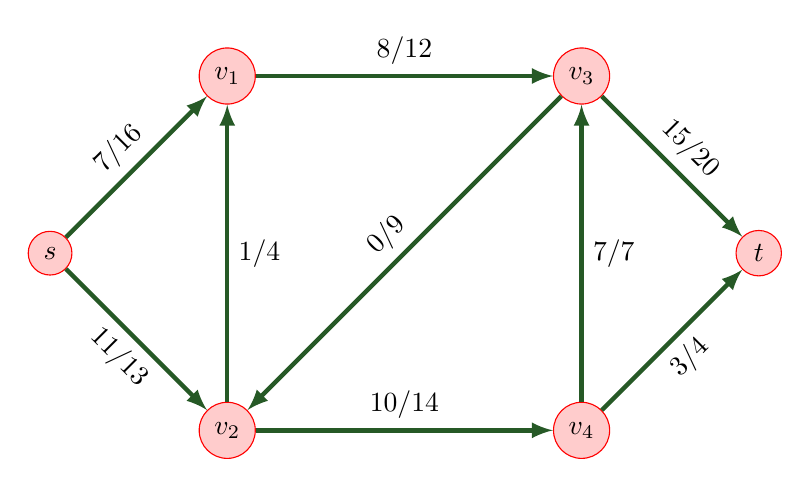
\begin{tikzpicture}[x=1.5cm, y=1.5cm]
	%\fill (-3.2,0) circle (0.1pt)node[anchor=east] {$20$};
	%\fill (3.2,0) circle (0.1pt)node[anchor=west] {$-20$};
    \node[circle,draw=red,fill=red!20!] (v1) at (-1.5,1.5) {$v_1$};
    \node[circle,draw=red,fill=red!20!] (v3) at (1.5,1.5) {$v_3$};
    \node[circle,draw=red,fill=red!20!] (t) at (3,0) {$t$};
    \node[circle,draw=red,fill=red!20!] (v4) at (1.5,-1.5) {$v_4$};
    \node[circle,draw=red,fill=red!20!] (v2) at (-1.5,-1.5) {$v_2$};
    \node[circle,draw=red,fill=red!20] (s) at (-3,0) {$s$};
    \draw[color=zzttqq, ultra thick, -latex]  (s) edge node[rotate = 45, above,color=black]{7/16} (v1);
	\draw[color=zzttqq, ultra thick, -latex]  (s) edge node[rotate = -45, below,color=black]{11/13} (v2);
	\draw[-latex, color=zzttqq, ultra thick]  (v2) edge node[right,color=black]{1/4} (v1);
	\draw[-latex, color=zzttqq, ultra thick]  (v1) edge node[above,color=black]{8/12} (v3);
	\draw[-latex, color=zzttqq, ultra thick]  (v2) edge node[above,color=black]{10/14} (v4);
	\draw[-latex, color=zzttqq, ultra thick]  (v3) edge node[rotate=45,above,color=black]{0/9} (v2);
	\draw[-latex, color=zzttqq, ultra thick]  (v4) edge node[right,color=black]{7/7} (v3);
	\draw[-latex, color=zzttqq, ultra thick]  (v3) edge node[rotate=-45,above,color=black]{15/20} (t);
	\draw[-latex, color=zzttqq, ultra thick]  (v4) edge node[rotate=45,below,color=black]{3/4} (t);
\end{tikzpicture}\end{center}\end{figura}

En la \textbf{Figura 4.1} hemos representado una red de flujo $G=(V,E)$ con una función de flujo y sus capacidades. Veamos como queda su red residual $G_f$.

\begin{figura}\ \begin{center}\definecolor{zzttqq}{rgb}{0.15,0.35,0.15}

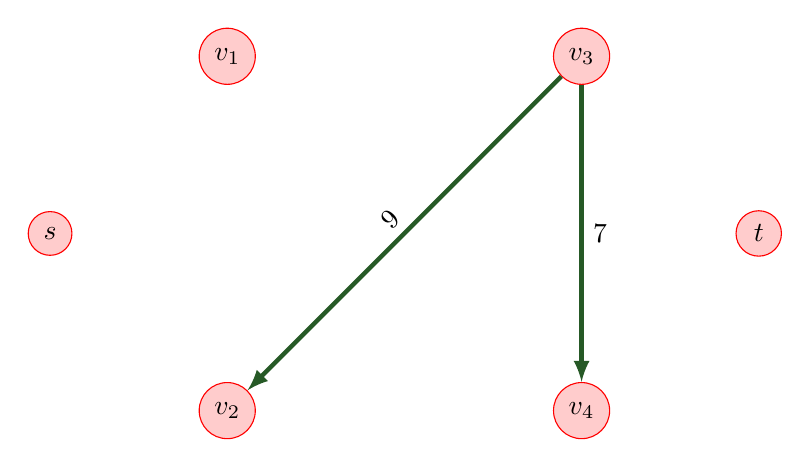
\begin{tikzpicture}[x=1.5cm, y=1.5cm]
	%\fill (-3.2,0) circle (0.1pt)node[anchor=east] {$20$};
	%\fill (3.2,0) circle (0.1pt)node[anchor=west] {$-20$};
    \node[circle,draw=red,fill=red!20!] (v1) at (-1.5,1.5) {$v_1$};
    \node[circle,draw=red,fill=red!20!] (v3) at (1.5,1.5) {$v_3$};
    \node[circle,draw=red,fill=red!20!] (t) at (3,0) {$t$};
    \node[circle,draw=red,fill=red!20!] (v4) at (1.5,-1.5) {$v_4$};
    \node[circle,draw=red,fill=red!20!] (v2) at (-1.5,-1.5) {$v_2$};
    \node[circle,draw=red,fill=red!20] (s) at (-3,0) {$s$};
    \DoubleLine{s}{v1}{latex-, color=zzttqq, ultra thick}{7}{-latex, color=zzttqq, ultra thick}{9}
    \DoubleLine{s}{v2}{latex-, color=zzttqq, ultra thick}{11}{-latex, color=zzttqq, ultra thick}{2}
    \DoubleLine{v2}{v1}{latex-, color=zzttqq, ultra thick}{1}{-latex, color=zzttqq, ultra thick}{3}
    \DoubleLine{v1}{v3}{latex-, color=zzttqq, ultra thick}{8}{-latex, color=zzttqq, ultra thick}{4}
    \DoubleLine{v2}{v4}{latex-, color=zzttqq, ultra thick}{10}{-latex, color=zzttqq, ultra thick}{4}
	%\draw[-latex, color=zzttqq, ultra thick]  (v2) edge node[above,color=black]{10/14} (v4);
	\draw[-latex, color=zzttqq, ultra thick]  (v3) edge node[rotate=45,above,color=black]{9} (v2);
	\draw[-latex, color=zzttqq, ultra thick]  (v3) edge node[right,color=black]{7} (v4);
    \DoubleLine{v3}{t}{latex-, color=zzttqq, ultra thick}{15}{-latex, color=zzttqq, ultra thick}{5}
	\DoubleLine{v4}{t}{latex-, color=zzttqq, ultra thick}{3}{-latex, color=zzttqq, ultra thick}{1}
\end{tikzpicture}\end{center}\end{figura}

En la \textbf{Figura 4.2} tenemos representado el grafo residual $G_f$ derivado del grafo $G$ y su función de flujo $f$.
\newpage
\begin{figura}\ \begin{center}\definecolor{zzttqq}{rgb}{0.15,0.35,0.15}

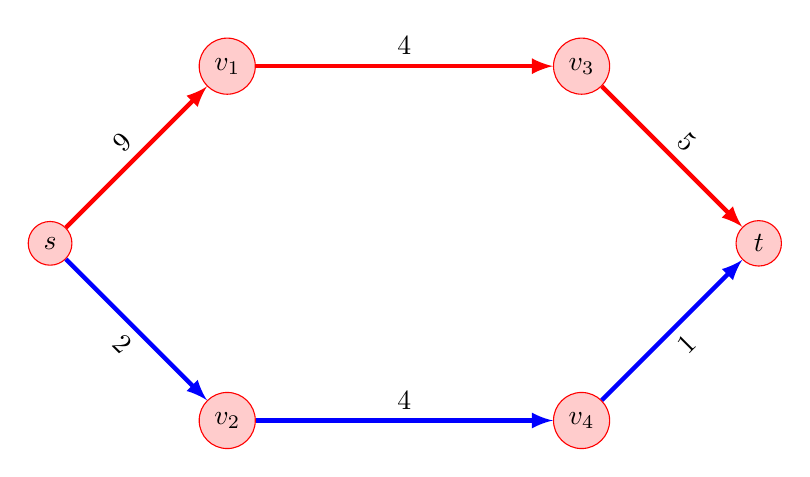
\begin{tikzpicture}[x=1.5cm, y=1.5cm]
	%\fill (-3.2,0) circle (0.1pt)node[anchor=east] {$20$};
	%\fill (3.2,0) circle (0.1pt)node[anchor=west] {$-20$};
    \node[circle,draw=red,fill=red!20!] (v1) at (-1.5,1.5) {$v_1$};
    \node[circle,draw=red,fill=red!20!] (v3) at (1.5,1.5) {$v_3$};
    \node[circle,draw=red,fill=red!20!] (t) at (3,0) {$t$};
    \node[circle,draw=red,fill=red!20!] (v4) at (1.5,-1.5) {$v_4$};
    \node[circle,draw=red,fill=red!20!] (v2) at (-1.5,-1.5) {$v_2$};
    \node[circle,draw=red,fill=red!20] (s) at (-3,0) {$s$};
    \draw[color=red, ultra thick, -latex]  (s) edge node[rotate = 45, above,color=black]{9} (v1);
	\draw[color=blue, ultra thick, -latex]  (s) edge node[rotate = -45, below,color=black]{2} (v2);
	\draw[-latex, color=red, ultra thick]  (v1) edge node[above,color=black]{4} (v3);
	\draw[-latex, color=blue, ultra thick]  (v2) edge node[above,color=black]{4} (v4);
	\draw[-latex, color=red, ultra thick]  (v3) edge node[rotate=-45,above,color=black]{5} (t);
	\draw[-latex, color=blue, ultra thick]  (v4) edge node[rotate=45,below,color=black]{1} (t);
\end{tikzpicture}\end{center}\end{figura}

En la \textbf{Figura 4.3} hemos dibujado dos cadenas de aumento (en rojo y azul respectivamente). Si denotamos el camino rojo como $p_1$, tenemos que $c_f(p_1)=4$ y que $f_{p_1}(s,v_1)=f_{p_1}(v_1,v_3)=f_{p_1}(v_3,t)=4$. Mientras que si denotamos el azul por $p_2$, obtenemos $c_f(p_2)=1$ y que $f_{p_2}(s,v_2)=f_{p_1}(v_2,v_4)=f_{p_1}(v_4,t)=1$. Nos quedaremos por ejemplo con el rojo y así surge el flujo de aumento $f\uparrow f_{p_2}$ presente en la \textbf{Figura 4.4}.

\begin{figura}\ \begin{center}\definecolor{zzttqq}{rgb}{0.15,0.35,0.15}

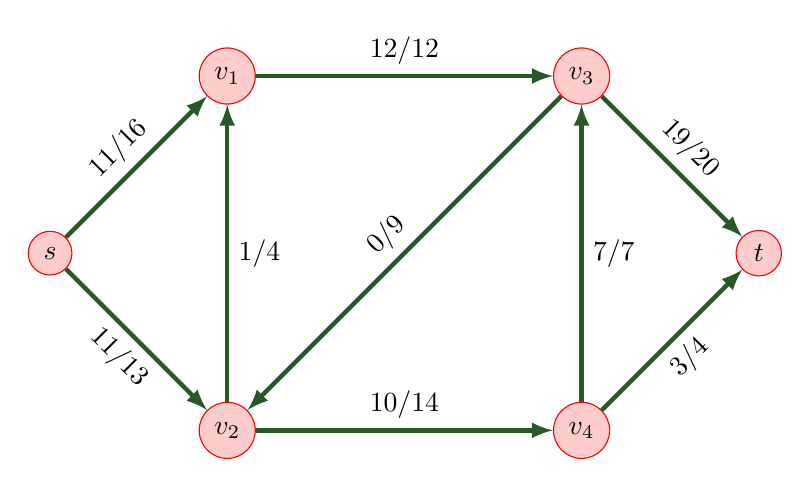
\begin{tikzpicture}[x=1.5cm, y=1.5cm]
	%\fill (-3.2,0) circle (0.1pt)node[anchor=east] {$20$};
	%\fill (3.2,0) circle (0.1pt)node[anchor=west] {$-20$};
    \node[circle,draw=red,fill=red!20!] (v1) at (-1.5,1.5) {$v_1$};
    \node[circle,draw=red,fill=red!20!] (v3) at (1.5,1.5) {$v_3$};
    \node[circle,draw=red,fill=red!20!] (t) at (3,0) {$t$};
    \node[circle,draw=red,fill=red!20!] (v4) at (1.5,-1.5) {$v_4$};
    \node[circle,draw=red,fill=red!20!] (v2) at (-1.5,-1.5) {$v_2$};
    \node[circle,draw=red,fill=red!20] (s) at (-3,0) {$s$};
    \draw[color=zzttqq, ultra thick, -latex]  (s) edge node[rotate = 45, above,color=black]{11/16} (v1);
	\draw[color=zzttqq, ultra thick, -latex]  (s) edge node[rotate = -45, below,color=black]{11/13} (v2);
	\draw[-latex, color=zzttqq, ultra thick]  (v2) edge node[right,color=black]{1/4} (v1);
	\draw[-latex, color=zzttqq, ultra thick]  (v1) edge node[above,color=black]{12/12} (v3);
	\draw[-latex, color=zzttqq, ultra thick]  (v2) edge node[above,color=black]{10/14} (v4);
	\draw[-latex, color=zzttqq, ultra thick]  (v3) edge node[rotate=45,above,color=black]{0/9} (v2);
	\draw[-latex, color=zzttqq, ultra thick]  (v4) edge node[right,color=black]{7/7} (v3);
	\draw[-latex, color=zzttqq, ultra thick]  (v3) edge node[rotate=-45,above,color=black]{19/20} (t);
	\draw[-latex, color=zzttqq, ultra thick]  (v4) edge node[rotate=45,below,color=black]{3/4} (t);
\end{tikzpicture}\end{center}\end{figura}

En este caso hemos aumentado de un flujo $|f|=18$ a $22$. Podríamos redibujar la nueva red residual del grafo $G$ resultante y continuar buscando otra cadena de aumento, así hasta que no encontráramos ninguna otra.
\newpage
\begin{figura}\ \begin{center}\definecolor{zzttqq}{rgb}{0.15,0.35,0.15}

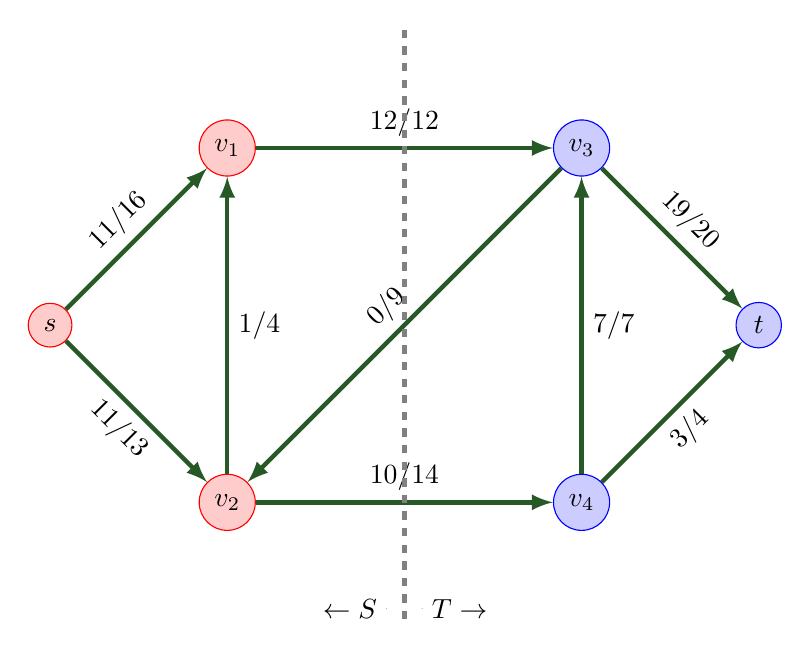
\begin{tikzpicture}[x=1.5cm, y=1.5cm]
	\fill (0.15,-2.4) circle (0.1pt)node[anchor=west] {$T\rightarrow$};
	\fill (-0.15,-2.4) circle (0.1pt)node[anchor=east] {$\leftarrow S$};
	\node[circle,draw=red,fill=red!20] (s) at (-3,0) {$s$};
    \node[circle,draw=red,fill=red!20!] (v1) at (-1.5,1.5) {$v_1$};
    \node[circle,draw=red,fill=red!20!] (v2) at (-1.5,-1.5) {$v_2$};
    
    \node[circle,draw=blue,fill=blue!20!] (v3) at (1.5,1.5) {$v_3$};
    \node[circle,draw=blue,fill=blue!20!] (v4) at (1.5,-1.5) {$v_4$};
    \node[circle,draw=blue,fill=blue!20!] (t) at (3,0) {$t$};
    
    \draw[color=zzttqq, ultra thick, -latex]  (s) edge node[rotate = 45, above,color=black]{11/16} (v1);
	\draw[color=zzttqq, ultra thick, -latex]  (s) edge node[rotate = -45, below,color=black]{11/13} (v2);
	\draw[-latex, color=zzttqq, ultra thick]  (v2) edge node[right,color=black]{1/4} (v1);
	\draw[-latex, color=zzttqq, ultra thick]  (v1) edge node[above,color=black]{12/12} (v3);
	\draw[-latex, color=zzttqq, ultra thick]  (v2) edge node[above,color=black]{10/14} (v4);
	\draw[-latex, color=zzttqq, ultra thick]  (v3) edge node[rotate=45,above,color=black]{0/9} (v2);
	\draw[-latex, color=zzttqq, ultra thick]  (v4) edge node[right,color=black]{7/7} (v3);
	\draw[-latex, color=zzttqq, ultra thick]  (v3) edge node[rotate=-45,above,color=black]{19/20} (t);
	\draw[-latex, color=zzttqq, ultra thick]  (v4) edge node[rotate=45,below,color=black]{3/4} (t);
	\draw[color=gray, ultra thick, dashed]  (0, 2.5) edge (0,-2.5);
\end{tikzpicture}\end{center}\end{figura}

Para finalizar con estos ejemplos, en la \textbf{Figura 4.5} hemos practicado un corte $(S,T)$ sobre el grafo de la \textbf{Figura 4.4}. Su flujo neto $f(S,T)=\stackbin[u\in S]{}\sum\stackbin[v\in T]{}\sum f(u,v)-\stackbin[u\in S]{}\sum\stackbin[v\in T]{}\sum f(v,u)=\\= f(v_1,v_3)+f(v_2,v_4)-f(v_3,v_2)=12+10-0=22$. Mientras que su capacidad de corte es $c(S,T)=\stackbin[u\in S]{}\sum\stackbin[v\in T]{}\sum c(u,v)=c(v_1,v_3)+c(v_2,v_4)=12+14=26$.

\subsection{Teorema del flujo máximo y corte mínimo}
\begin{teor} Sea $f$ un flujo en una red $G=(V,E)$ con una fuente $s$ y un sumidero $t$, entonces son equivalentes:
\begin{enumerate}[1)]
\item $f$ es máximo flujo en $G$.
\item La red residual $G_f$ no contiene cadenas de aumento.
\item $|f|=c(S,T)$ para cierto corte $(S,T)$ de $G$.
\end{enumerate}
\begin{proof}\ 
\begin{itemize}
\item (1 $\implies$ 2) Supongamos que no. Supongamos que $f$ es flujo máximo en $G$ y existe una cadena de aumento $p$ en $G_f$. Entonces existe una función de flujo $f_p$ en $G_f$ y por la \textbf{Proposición 4.2}, la función de flujo $f\uparrow f_p$ está bien definida sobre $G$ y $|f\uparrow f_p|=|f|+|f_p|>|f|$ lo que contradice que $f$ sea flujo máximo.
\newpage
\item (2 $\implies$ 3) Supongamos que no existen cadenas de aumento, esto es que no hay ningún camino de $s$ a $t$ en $G_f$. Definimos $S=\{v\in V\ |\ $existe un camino de $s$ a $v\}$, evidentemente $t\notin S$ puesto que no existe ningún camino de $s$ a $t$ y definimos $T=V\setminus S$. $(S,T)$ es un corte y para cada par $(u,v)$ con $u\in S, v\in T$, $(u,v)\notin E_f$, puesto que no existe un camino entre ellos. Tenemos que si $(u,v)\in E$, por lo anterior, $f(u,v)=c(u,v)$. Si $(v,u)\in E$, entonces $f(v,u)=0$ ya que en otro caso $(u,v)$ pertenecería a $E_f$ y esto no es posible. Así tenemos que\\ $f(S,T)=\stackbin[u\in S]{}\sum\stackbin[v\in T]{}\sum f(u,v)-\stackbin[u\in S]{}\sum\stackbin[v\in T]{}\sum f(v,u)=\stackbin[u\in S]{}\sum\stackbin[v\in T]{}\sum f(u,v)=\stackbin[u\in S]{}\sum\stackbin[v\in T]{}\sum c(u,v)=c(S,T)$.
\item (3 $\implies$ 1) Por la \textbf{Proposición 4.3} tenemos que $|f|\leq c(S,T)$ para cualquier corte $(S,T)$ de $G$, como $|f|= c(S,T)\implies f$ es máximo.
\end{itemize}
\end{proof}
\end{teor}

\subsection{Implementación en pseudocódigo del método Ford-Fulkerson y complejidad}

Para finalizar esta sección veamos un algoritmo del método \textbf{\textit{Ford-Fulkerson}} implementado en pseudocódigo. Como observaremos, el código es bastante simple.

\begin{algorithmic}[1]
\State /*********************
\State	* FordFulkerson ($G,s,t,f$)
\State *********************/
\For {cada arista $(u,v) \in G.E$}
	\State $f(u,v) = 0$
\EndFor
\While {$\exists p$ cadena de aumento en $G_f$}
	\State $c_f(p)=\min\{c_f(u,v)\ |\ (u,v)$ está en $p\}$
	\For {cada arista $(u,v)$ en $p$}
		\If {$(u,v)\in G.E$}
			\State $f(u,v) = f(u,v) +c_f(p)$
		\Else
			\State $f(u,v) = f(u,v) -c_f(p)$
		\EndIf
	\EndFor
\EndWhile
\end{algorithmic}
\ 

Para la búsqueda del camino podemos utilizar uno de los algoritmos de búsqueda en profundidad sobre el grafo $G_f$ vistos en clase. Recordemos que el coste de cualquiera de estas búsquedas tiene $\mathcal{O}(V+E')$ que podemos reducir a $\mathcal{O}(E')$, puesto que en general tendremos muchas más aristas que vértices. Además recordemos que $\card(E')\leq2\cdot\card(E)$, luego $\mathcal{O}(E')=\mathcal{O}(2E)=\mathcal{O}(E)$.
Por último, el número máximo de veces que buscaremos si hay o no este camino será cuando lleguemos a alcanzar el flujo máximo, es decir, $|f|$. Luego el orden de \textbf{\textit{Ford-Fulkerson}} puede ser definido como $\mathcal{O}(|f|E)$.